%%%%%%%%%%%%%%%%%%%%%%%%%%%%%%%%%%%%%%%%%
% Arsclassica Article
% LaTeX Template
% Version 1.1 (10/6/14)
%
% This template has been downloaded from:
% http://www.LaTeXTemplates.com
%
% Original author:
% Lorenzo Pantieri (http://www.lorenzopantieri.net) with extensive modifications by:
% Vel (vel@latextemplates.com)
%
% License:
% CC BY-NC-SA 3.0 (http://creativecommons.org/licenses/by-nc-sa/3.0/)
%
%%%%%%%%%%%%%%%%%%%%%%%%%%%%%%%%%%%%%%%%%

%----------------------------------------------------------------------------------------
%	PACKAGES AND OTHER DOCUMENT CONFIGURATIONS
%----------------------------------------------------------------------------------------

\documentclass[
10pt, % Main document font size
a4paper, % Paper type, use 'letterpaper' for US Letter paper
oneside,
%twocolumn, % One page layout (no page indentation)
%twoside, % Two page layout (page indentation for binding and different headers)
headinclude,footinclude, % Extra spacing for the header and footer
BCOR 0mm, % Binding correction
]{scrartcl}

%%%%%%%%%%%%%%%%%%%%%%%%%%%%%%%%%%%%%%%%%
% Arsclassica Article
% Structure Specification File
%
% This file has been downloaded from:
% http://www.LaTeXTemplates.com
%
% Original author:
% Lorenzo Pantieri (http://www.lorenzopantieri.net) with extensive modifications by:
% Vel (vel@latextemplates.com)
%
% License:
% CC BY-NC-SA 3.0 (http://creativecommons.org/licenses/by-nc-sa/3.0/)
%
%%%%%%%%%%%%%%%%%%%%%%%%%%%%%%%%%%%%%%%%%

%----------------------------------------------------------------------------------------
%	REQUIRED PACKAGES
%----------------------------------------------------------------------------------------

\usepackage[
nochapters, % Turn off chapters since this is an article        
beramono, % Use the Bera Mono font for monospaced text (\texttt)
eulermath,% Use the Euler font for mathematics
pdfspacing, % Makes use of pdftex’ letter spacing capabilities via the microtype package
dottedtoc % Dotted lines leading to the page numbers in the table of contents
]{classicthesis} % The layout is based on the Classic Thesis style

\usepackage{arsclassica} % Modifies the Classic Thesis package

\usepackage[T1]{fontenc} % Use 8-bit encoding that has 256 glyphs

\usepackage[utf8]{inputenc} % Required for including letters with accents



\usepackage{enumitem} % Required for manipulating the whitespace between and within lists

\usepackage{lipsum} % Used for inserting dummy 'Lorem ipsum' text into the template

\usepackage{graphicx}
\usepackage{caption}
\usepackage{subcaption} % Required for creating figures with multiple parts (subfigures)

\usepackage{amsmath,amssymb,amsthm} % For including math equations, theorems, symbols, etc

\usepackage{varioref} % More descriptive referencing

\usepackage{listings}
\usepackage{color}

\definecolor{dkgreen}{rgb}{0,0.6,0}
\definecolor{gray}{rgb}{0.5,0.5,0.5}
\definecolor{mauve}{rgb}{0.58,0,0.82}

\lstset{frame=tb,
  language=Java,
  aboveskip=3mm,
  belowskip=3mm,
  showstringspaces=false,
  columns=flexible,
  basicstyle={\small\ttfamily},
  numbers=none,
  numberstyle=\tiny\color{gray},
  keywordstyle=\color{blue},
  commentstyle=\color{dkgreen},
  stringstyle=\color{mauve},
  breaklines=true,
  breakatwhitespace=true,
  tabsize=3
}

%----------------------------------------------------------------------------------------
%	THEOREM STYLES
%---------------------------------------------------------------------------------------

\theoremstyle{definition} % Define theorem styles here based on the definition style (used for definitions and examples)
\newtheorem{definition}{Definition}

\theoremstyle{plain} % Define theorem styles here based on the plain style (used for theorems, lemmas, propositions)
\newtheorem{theorem}{Theorem}

\theoremstyle{remark} % Define theorem styles here based on the remark style (used for remarks and notes)

%----------------------------------------------------------------------------------------
%	HYPERLINKS
%---------------------------------------------------------------------------------------

\hypersetup{
%draft, % Uncomment to remove all links (useful for printing in black and white)
colorlinks=true, breaklinks=true, bookmarks=true,bookmarksnumbered,
urlcolor=webbrown, linkcolor=RoyalBlue, citecolor=webgreen, % Link colors
pdftitle={}, % PDF title
pdfauthor={\textcopyright}, % PDF Author
pdfsubject={}, % PDF Subject
pdfkeywords={}, % PDF Keywords
pdfcreator={pdfLaTeX}, % PDF Creator
pdfproducer={LaTeX with hyperref and ClassicThesis} % PDF producer
} % Include the structure.tex file which specified the document structure and layout

\hyphenation{Fortran hy-phen-ation} % Specify custom hyphenation points in words with dashes where you would like hyphenation to occur, or alternatively, don't put any dashes in a word to stop hyphenation altogether

\usepackage{geometry}
\geometry{
  left=3cm,
  right=3cm,
  top=2cm,
  bottom=4cm,
  bindingoffset=5mm
}

%----------------------------------------------------------------------------------------
%	TITLE AND AUTHOR(S)
%----------------------------------------------------------------------------------------

\title{\normalfont\spacedallcaps{Visual SceneMaker integration in Blender}} % The article title

\author{\spacedlowsmallcaps{Timo Gühring \& Janna Herrmann}} % The article author(s) - author affiliations need to be specified in the AUTHOR AFFILIATIONS block

\date{} % An optional date to appear under the author(s)

%----------------------------------------------------------------------------------------

\begin{document}

%----------------------------------------------------------------------------------------
%	HEADERS
%----------------------------------------------------------------------------------------

\renewcommand{\sectionmark}[1]{\markright{\spacedlowsmallcaps{#1}}} % The header for all pages (oneside) or for even pages (twoside)
%\renewcommand{\subsectionmark}[1]{\markright{\thesubsection~#1}} % Uncomment when using the twoside option - this modifies the header on odd pages
\lehead{\mbox{\llap{\small\thepage\kern1em\color{halfgray} \vline}\color{halfgray}\hspace{0.5em}\rightmark\hfil}} % The header style

\pagestyle{scrheadings} % Enable the headers specified in this block

%----------------------------------------------------------------------------------------
%	TABLE OF CONTENTS & LISTS OF FIGURES AND TABLES
%----------------------------------------------------------------------------------------

\maketitle % Print the title/author/date block

%----------------------------------------------------------------------------------------
%	ABSTRACT
%----------------------------------------------------------------------------------------

%\section*{Abstract} % This section will not appear in the table of contents due to the star (\section*)


%----------------------------------------------------------------------------------------
%	INTRODUCTION
%----------------------------------------------------------------------------------------

\section{Introduction}

In the context of the seminar "Software design and architectures for interactive avatars: a hands-on approach" we developed an integration of Visual SceneMaker\footnote{\url{http://scenemaker.dfki.de/}} in Blender \footnote{\url{https://www.blender.org/}}.
Visual SceneMaker is a software for creating interactive presentations specialized to users with no programming experience and Blender is a open source 3D creation suite.\\
The integration is mainly about avatar animation. It is possible, to create scenes in Visual SceneMaker with actors, speeches and actions. These defined action and speech activities will be sent via a UDP socket connection to Blender, in which actors perform the actions whenever a message from SceneMaker is retrieved. An actor can be an avatar itself or objects in the environment, for example a light that can be turned on, off or dimmed.
%----------------------------------------------------------------------------------------
%	MANUAL
%----------------------------------------------------------------------------------------

\section{Manual}
In order to make the integration of Visual SceneMaker in Blender work, please follow the steps below:
\begin{enumerate}[noitemsep] % [noitemsep] removes whitespace between the items for a compact look
\item Change to your terminal.
\item Execute the following commands inside the terminal:
\begin{lstlisting}
$ git clone git@github.com:JeannedArk/seminarsmcomm.git
$ cd ./seminarsmcomm
$ sh start.sh
\end{lstlisting}
\item Close the Blender window with the default setup. Select the Blender window with Anna as character. Press „P“ to start the game mode.
\item Visual SceneMaker will automatically open. Click „Open a project“ > select the „UDPForwarder“ project provided in the cloned repository > click the „select“ button > click the Play button
\item Now you can see the character moving in Blender to the corresponding actions defined by the graph.
\end{enumerate}
\begin{figure}
\centering
\begin{subfigure}{.5\textwidth}
  \centering
  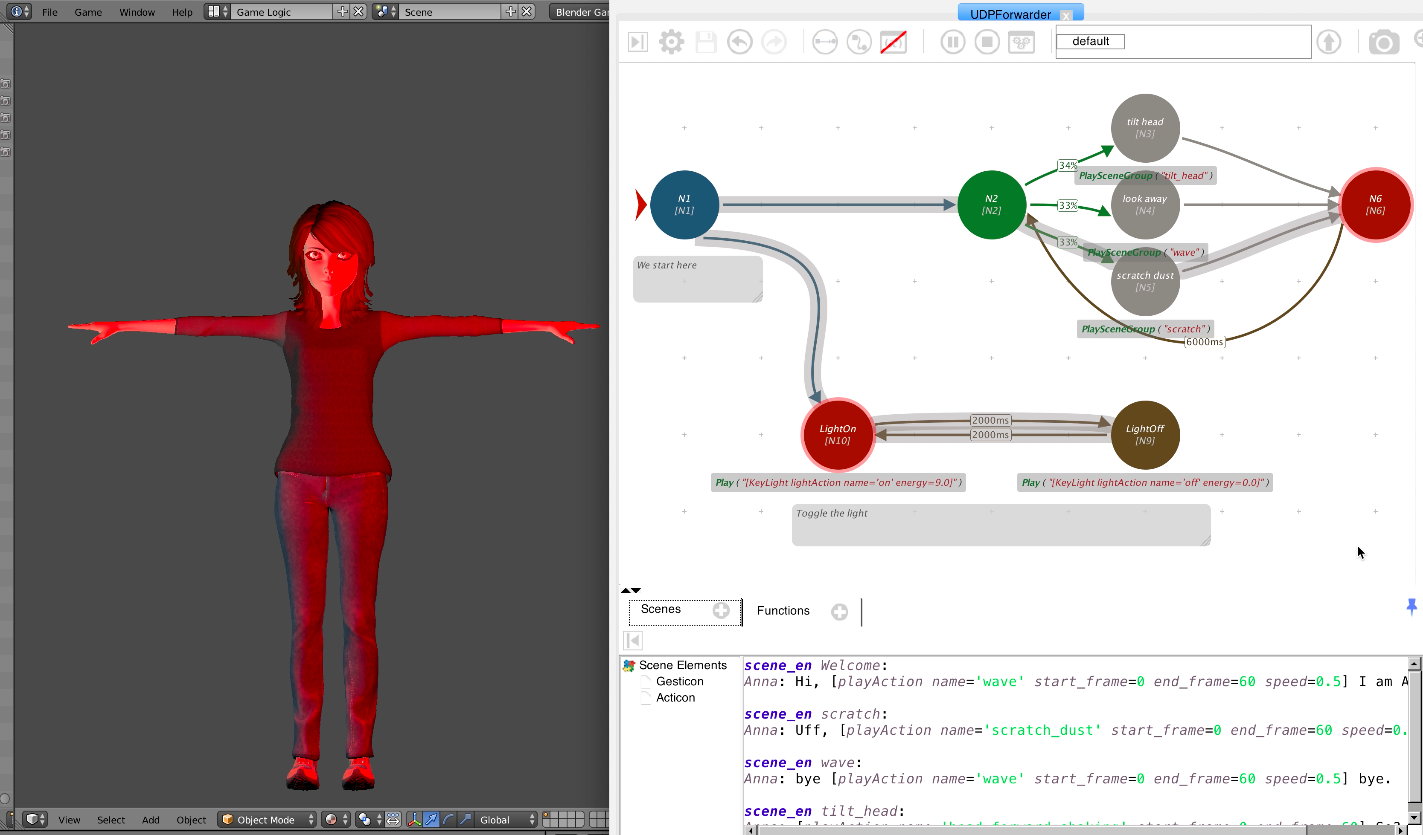
\includegraphics[width=.9\linewidth]{Figures/lightsOn.png}
  \caption{Scene with lights on.}
  \label{fig:sub1}
\end{subfigure}%
\begin{subfigure}{.5\textwidth}
  \centering
  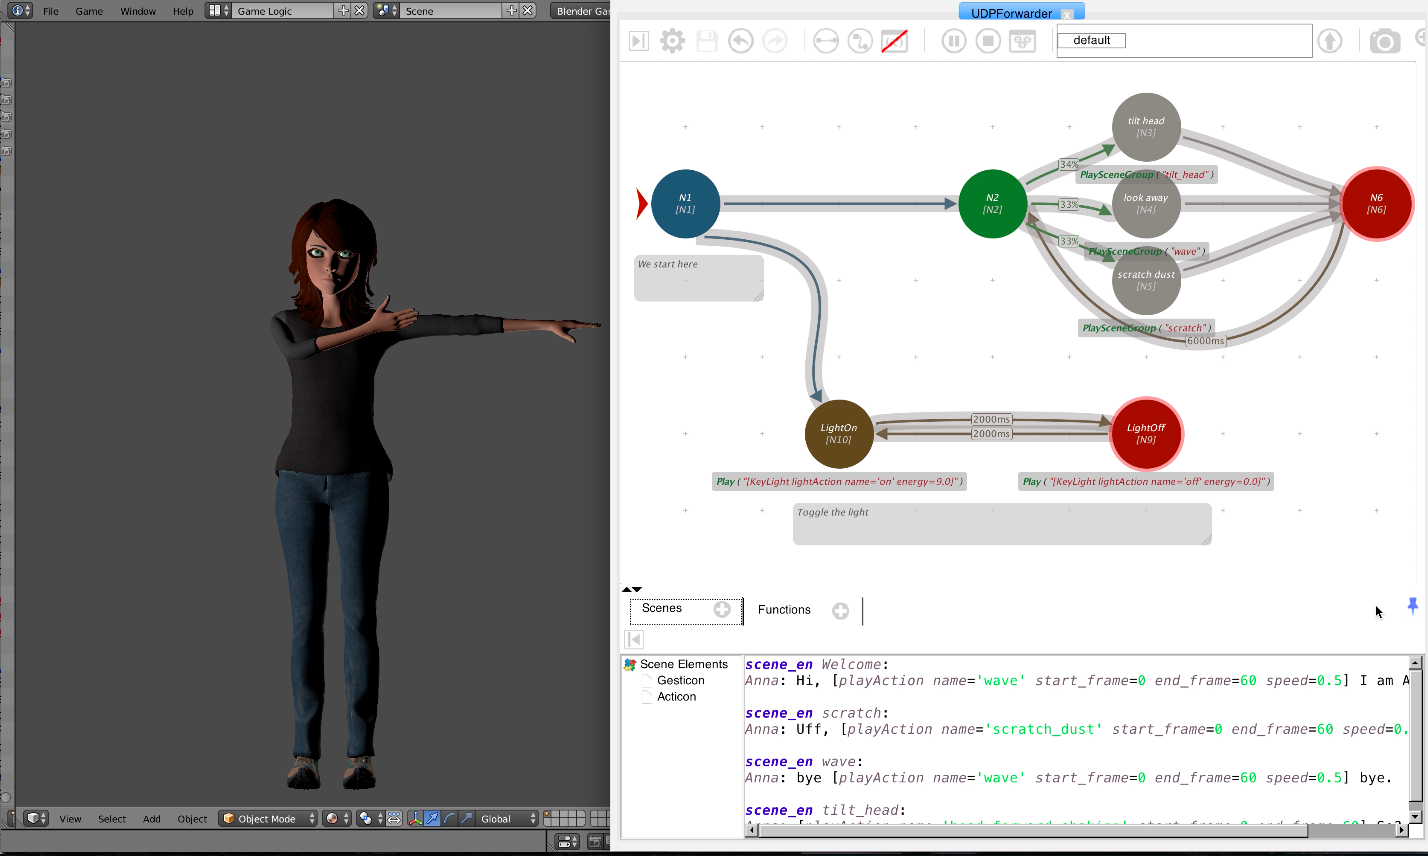
\includegraphics[width=.9\linewidth]{Figures/lightsOff.png}
  \caption{Scene with lights off and performing action "scratch dust"}
  \label{fig:sub2}
\end{subfigure}
\caption{The avatar in Blender on the right and the corresponding scene in Visual SceneMaker on the left}
\label{fig:test}
\end{figure}

%------------------------------------------------

\section{Implementation}
Our implementation presupposes some constraints especially in the naming of actions and avatars in order to work correctly.
One constraint is, that the name of avatar, which should perform the action, is the same in Blender and Visual SceneMaker. Another one is, that the actions must be named the same in both programs.
\subsection*{Design Choices}
Together with our implementation we had to make several design choices.\\
We decided to use JSON as a transport format, because it is a well known and light-weight format. Another very important fact is, that there is no need for manual parsing of the retrieved string messages on python side.\\
Furthermore we used a command pattern to execute the activities, because of the high grade of flexibility and dynamic and therefore it builds the base for an easy maintenance and extension in the future. Programmatically spoken the command pattern bewares the concept of separation of concerns.
\subsection*{Visual SceneMaker}
To make the communication work, there is a class implemented in Visual SceneMaker called UDPForwarder. It parses the information from the scenes in SceneMaker in action activities and speech activities and sends them, formalized as strings in JSON representation to the localhost address on port 2300. This can be easily changed to other desired addresses and ports.
\subsection*{Blender}
In Blender we needed an abstract class which represents the activities modeled in SceneMaker. This class is implemented by the two subclasses  ActionActivity and SpeechActivity, to be consistent to the SceneMaker implementation. For executing the activities we used the command pattern. Currently, only the executing of ActionActivities is implemented.\\
For the communication we implemented a module called SceneMakerCommunication. Here, the data from the current running Visual SceneMaker instance is recieved and mapped to the ActionActivity or the SpeechActivity class. For communication it creates a socket with the defined configuration. The retrieved
activities will be further propagated to Blender. The retrieving of the data is outsourced to another thread.\\
Incoming data is stored by this thread in a threadsafe queue. The update method in the communication module pops the oldest activity from the queue and executes it, if existing. Additionally the action is only played if no other action of this object is currently not playing an action. Otherwise actions would interfere with each other and stop playing the old one. Therefore we had to extend the standard python 3 threadsafe queue with a peek operation, because the standard queue only implements a get function, which automatically pops the action. The PeekQueue allows us to check the potential next action in the queue without removing it.

%----------------------------------------------------------------------------------------
%	RESULTS AND DISCUSSION
%----------------------------------------------------------------------------------------

\section{Results and Future Work}
So far, only action activities of the actors were implemented as actions in Blender. Speech activities are currently sent and recognized as speech, but not interpreted as actions by the avatars in Blender. In order to do that, an integration of a Text-to-Speech software, like for example MaryTTS in Blender would be necessary. \\
For evaluation, we performed a stress test with a scene in which events will be sent every 5 ms. The result showed that it performed very fast on a local machine, so that there was no recognizable delay in receiving the events. Also the communication protocol can be variably extended andsent to arbitrary network addresses.\\
Altogether the result of our work is a flexible and powerful solution to communicate between Visual SceneMaker and Blender.


\end{document}